% 第4章
%!TEX root = main.tex

%%%%%%%%%%%%%%%%%%%%%%%%
\chapter{パラメータ同定}
\label{sys_id}
%%%%%%%%%%%%%%%%%%%%%%%%

本章では,開発機体を用いた実験で得た飛行データをもとに,モデル内の未知パラメータを同定する手順および手法について述べる.その後,実際の実機実験によるデータの取得と,同定の結果を述べる.

高次元モデルを用いて正確なパラメータ推定を行なうことは困難であるため,ここまでに記述した低次元モデル,中でも縦運動にのみ注目しさらに低次元化したモデルを用いて推定を行なう.ただし,縦運動と横運動に分ける際に,それぞれの干渉を無視した条件を与えることになる.そのため,単純に低次元化しただけでは欲しい実験データ取得の困難性が残る.そこで,プロの操縦者に協力してもらい,できる限り各運動に限定したデータ取得を行なっている.\label{da}

%%%%%%%%%%%%%%%%%%%%%%%%
\section{データの前処理}
\label{sec:data_prepro}
%%%%%%%%%%%%%%%%%%%%%%%%

本節では,取得したログデータの前処理について述べる.前処理としては,得られたデータを計算に必要な値に変換する処理と,データのフィルタリングに大きく分けられる.

\subsection{対地速度の補正}

開発機体には,3軸方向の角速度および加速度を検出するセンサとして,慣性計測装置(Inertial Measurement Unit, IMU)が搭載されている.IMUから飛行ログデータとして得られる値は,当然センサが取り付けられている位置における値である.しかし,各運動モデルは機体座標系の原点を基準として構成されているため,原点位置にセンサを取り付けることができない場合,その分の補正が必要となる.ここでは,取り付け位置によって変化する速度の補正について述べる.開発機体においては,Fig. \ref{fig:location_IMU}に示す位置に取り付けられている.このとき,Fig. \ref{fig:IMU_position}のように設定し,センサ取り付け位置での対地速度を$\mbox{\boldmath $V_p$}$とすると,機体軸原点の対地速度\mbox{\boldmath $V_g$}は
\begin{equation}
  \mbox{\boldmath $V_g$} \triangleq \dfrac{d}{dt}\mbox{\boldmath $R_{B}$} = \dfrac{d}{dt}(\mbox{\boldmath $R_{p}$} + \mbox{\boldmath $R_{pB}$}) =  \mbox{\boldmath $V_p$}+\mbox{\boldmath $\dot{R}_{pB}$}
\end{equation}
で与えられる.つまり,$\mbox{\boldmath $\dot{R}_{pB}$}$によってセンサ位置によるずれを補正することになる.このベクトルの機体座標表現は,$\mbox{\boldmath $R_{pB}$}$がセンサから機体軸原点に向けたベクトルであることに注意して
\begin{equation}
  \mbox{\boldmath $\dot{R}_{pB}$} = \mbox{\boldmath $\omega$}\times\mbox{\boldmath $R_{pB}$} =
  \left[
    \begin{array}{ccc}
      p \\
      q \\
      r
    \end{array}
  \right] \times
  \left[
    \begin{array}{ccc}
      -l_{px} \\
      0 \\
      l_{pz}
    \end{array}
  \right] =
  \left[
    \begin{array}{ccc}
      ql_{pz} \\
      -rl_{px} - pl_{pz} \\
      ql_{px}
    \end{array}
  \right]
\end{equation}
と計算できる.

\begin{figure}[htbp]
	\begin{center}
		\begin{tabular}{c}
			\begin{minipage}{0.5\hsize}
				\begin{center}
					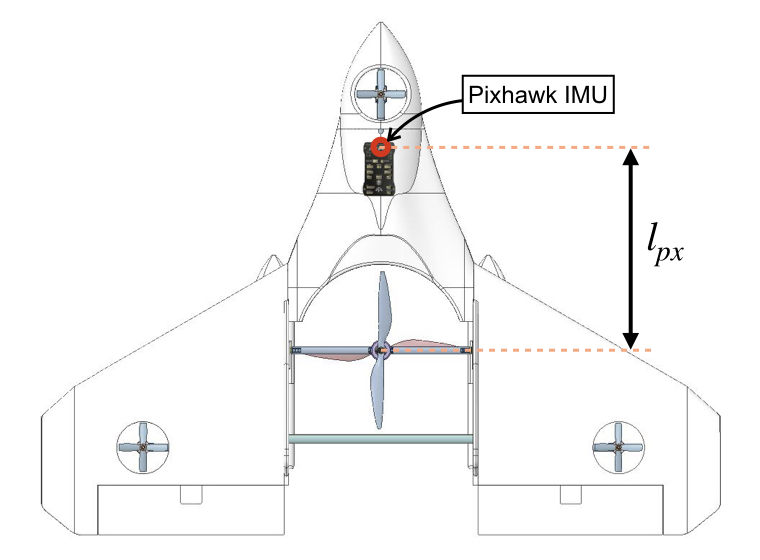
\includegraphics[clip,width=7.0cm,bb=0 0 760 560]{./z_figure_files/chapter4/1_location_IMU.jpeg}
					\caption{Location of IMU}
					\label{fig:location_IMU}
				\end{center}
			\end{minipage}
			\begin{minipage}{0.5\hsize}
				\begin{center}
					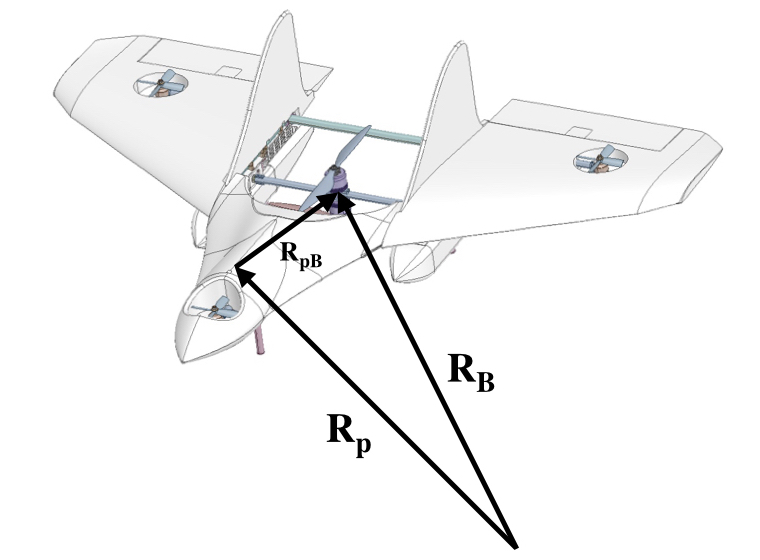
\includegraphics[clip,width=7.0cm,bb=0 0 760 560]{./z_figure_files/chapter4/2_IMU_position.jpeg}
					\caption{Position correction vector}
					\label{fig:IMU_position}
				\end{center}
			\end{minipage}
		\end{tabular}
	\end{center}
\end{figure}

\subsection{風の影響の補正}

実験は,屋外で風のある環境下で行なう.対気速度の測定のために,機首先端にピトー管が取り付けられているが,回転翼機モードでの飛行時は測定誤差が大きいことが分かっている.そこで,Fig. \ref{fig:wind_measure}に示すように,風速計を実験地点付近に機体の進行方向と同じ向きで設置し,風速を測定した.風速計の値は時々刻々変化するが,風速が一定に近い時間帯で実験を行ない,その時間帯のおおよその平均風速を測定値とした.データ処理時には,この測定値の一定風が吹いていると仮定し,機体の対地速度,および機体姿勢のログデータを用いて,\ref{sec:wind_speed}小節の通り対気速度を計算する.

\begin{figure}[H]
	\centering
	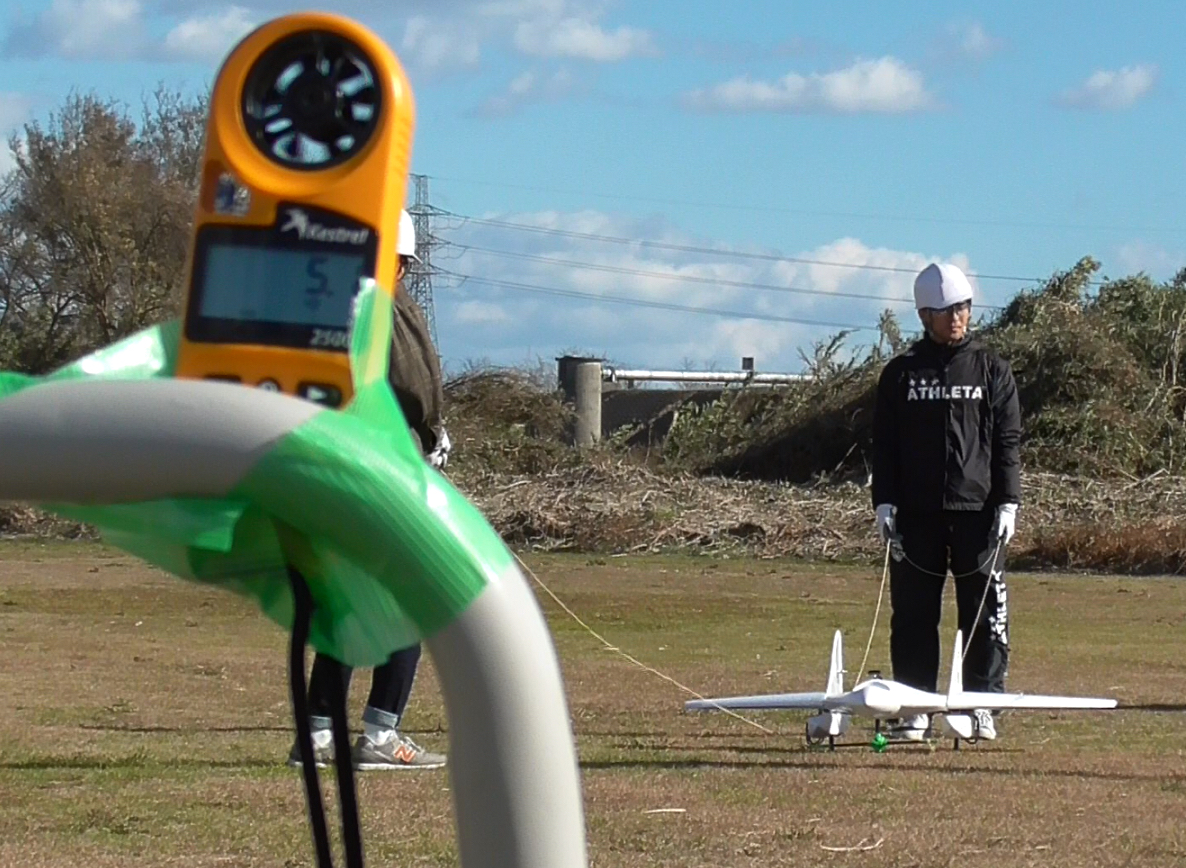
\includegraphics[clip,width=10.0cm,bb=0 0 1250 750]{./z_figure_files/chapter4/wind_measure.jpeg}
	\caption{Wind measurement}
	\label{fig:wind_measure}
\end{figure}


\subsection{算出が必要なデータ}

計算に必要だがログデータから直接得られない値の算出方法について述べる.具体的には,角加速度$\mbox{\boldmath $\dot{\omega}$}$と迎角速度$\dot{\alpha}$である.加えて,機体の加速度$\mbox{\boldmath $\dot{V_g}$}$は,ログデータからも直接得られるが,誤差が大きいため計算により求めている.それぞれ機体の速度$\mbox{\boldmath $V_g$}$,角速度$\mbox{\boldmath $\omega$}$,および迎角$\alpha$はログデータから得られるため,これらの差分から計算する.時間遅れを考慮し中心差分法を用いて,例として$\dot{u}$について表記すると
\begin{equation}
  \dot{u}_{[k]} = \dfrac{u_{[k+1]}-u_{[k-1]}}{2\Delta t}
\end{equation}
のように計算できる\cite{kawata}.$\Delta t$はログデータのサンプリング間隔であり,$k=1,2,3\hdots,n$はログデータのステップ数を表す.ただし,計算することができない左右境界の値は,ログデータから直接取得した値を採用する.同様に他の値についても計算で求める.

\subsection{各ロータ出力の評価}

メインロータおよびサブロータは,ログデータから得られる指令値(PWM値)を変換することによって推力値を得られる.この変換は,実験室内での予備実験により得られた測定結果から,計算結果と実際の推力との差が小さくなるように工夫して概算している.この概算の詳細は,\cite{yoshikawa}に示されている通りである.

\subsection{データのフィルタリング}
\label{sec:filter}

センサで取得したログデータには,様々なノイズが含まれているためそのままでは使えず,必要な信号成分だけを取り出すための処理を施す必要がある.そこで有効となるのが周波数によるフィルタリングである.パラメータ推定を行なう前に,フィルタリングによりデータの誤差を少なくしておかなければ,推定結果に余計な誤差が生じてしまう\cite{klein}.

そこで,後に\ref{sec:analyze}節で述べる解析結果から,おおよその機体の固有振動数を算出し,入力や制御の周波数も考慮して,ログデータに対して$10\mathrm{[Hz]}$をカットオフ周波数としたローパスフィルタをかけた.サンプリング間隔は$0.02\mathrm{[s]}$であるから,サンプリング周波数は$50\mathrm{[Hz]}$である.フィルタの実現には高速フーリエ変換(Fast Fourier Transform, FFT)を用いた.FFTによる周波数領域の解析の例として,後に\ref{sec:analyze}節でも触れる入力データの解析結果をFig. \ref{fig:f_input}に示す.左側に時系列データ,右側にFFTの解析結果を表示している.機首上サブロータの指令値を例としている.また,フィルタリング前後でどれだけノイズが除去されているかは,付録として載せることにする.

% ある実験データのピッチ角速度を例に,Fig. \ref{fig:f_filter}に示す.

\begin{figure}[H]
	\centering
	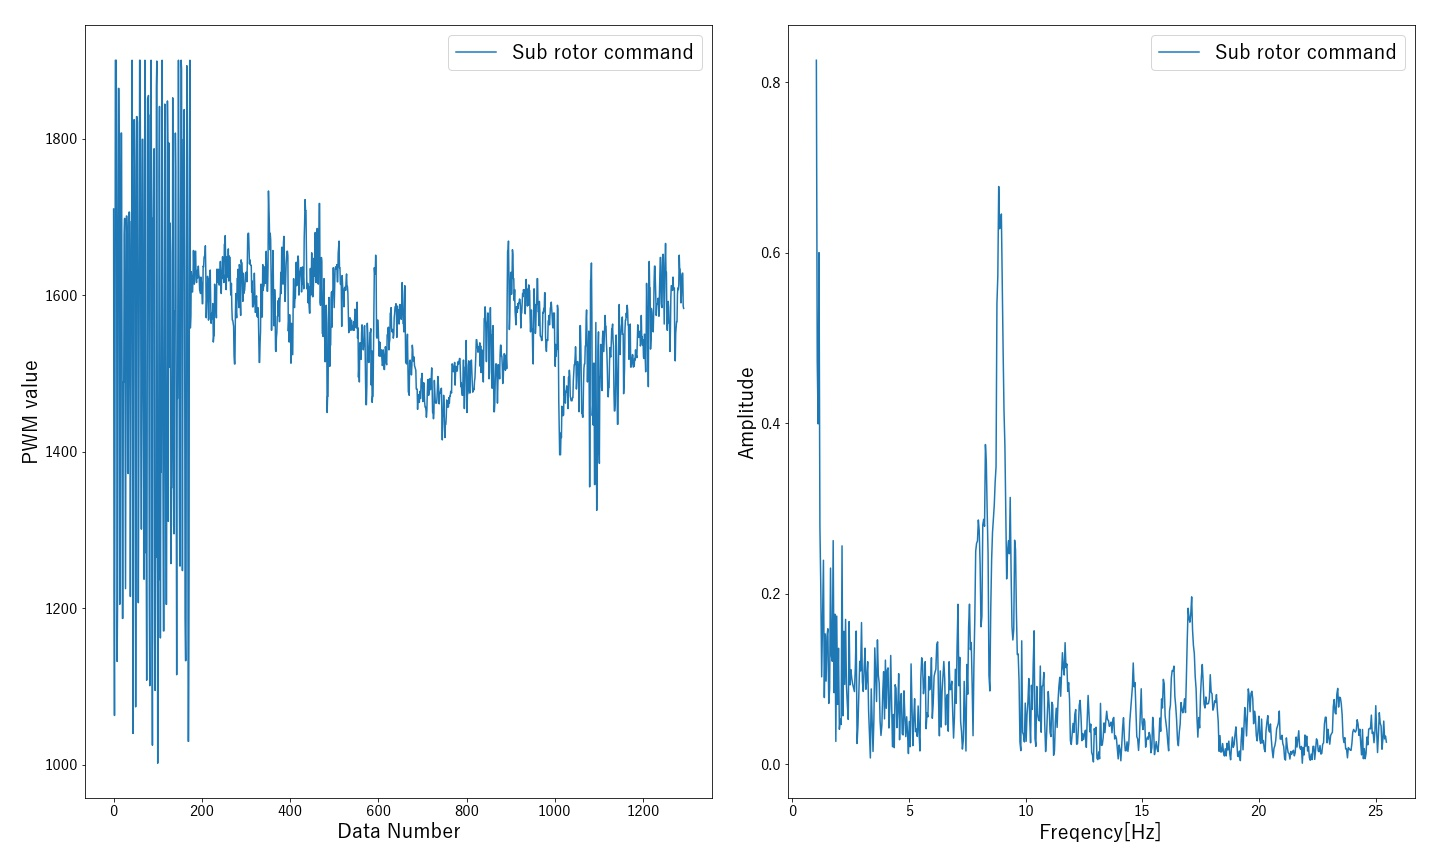
\includegraphics[clip,width=13.0cm,bb=0 0 1440 864]{./z_figure_files/chapter4/sub_input.jpeg}
	\caption{FFT analysis of sub rotor command}
	\label{fig:f_input}
\end{figure}

% \begin{figure}[H]
% 	\centering
% 	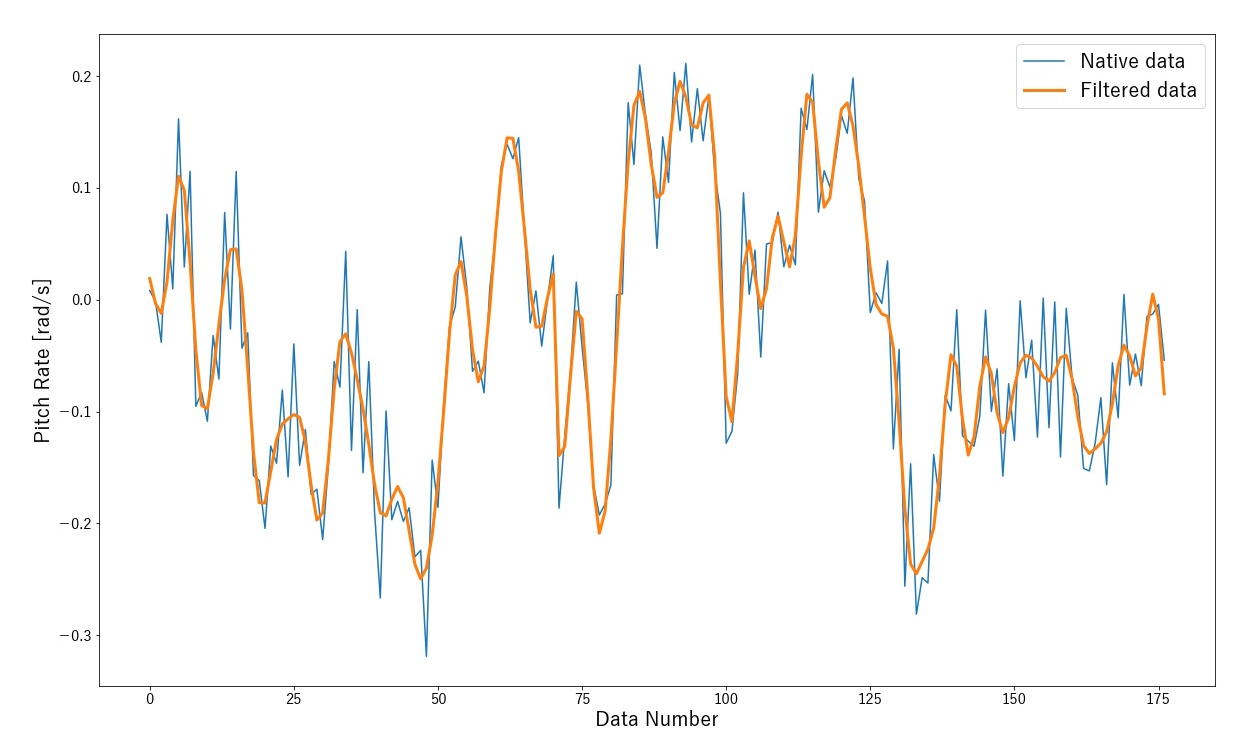
\includegraphics[clip,width=13.0cm,bb=0 0 1250 750]{./z_figure_files/chapter4/3_filter.jpeg}
% 	\caption{Filter pitch rate}
% 	\label{fig:f_filter}
% \end{figure}


% 補正が必要なデータとして,次の項目が挙げられる.
% \begin{itemize}
% \item[(1)]センサ取り付け位置の補正
% \item[(2)]風の影響の補正
% \item[(3)]各ロータ出力の評価
% \item[(4)]気温や気圧による気体密度変化の考慮
% \end{itemize}



%%%%%%%%%%%%%%%%%%%%%%%%%%%%%%
\section{パラメータの推定手法}
\label{sec:param_i}
%%%%%%%%%%%%%%%%%%%%%%%%%%%%%%

まず,モデル内の未知パラメータについて述べる.\ref{sec:lng_non_linear}小節に示したモデルにおいて,空気力項に未知パラメータが含まれる.ただし,\ref{sec:airspeed_airf}小節の空気力モデル式については,計算の際に式を変形して
\begin{equation}
  \left\{
  \begin{align}
    L &= \dfrac{1}{2}\rho {V_a}^2 S C_L^{\prime}, \quad C_L^{\prime} = \dfrac{L}{\frac{1}{2}\rho {V_a}^2 S} \\[5pt]
    D &= \dfrac{1}{2}\rho {V_a}^2 S C_D^{\prime}, \quad C_D^{\prime} = \dfrac{D}{\frac{1}{2}\rho {V_a}^2 S} \\[5pt]
    M_a &= \dfrac{1}{2}\rho {V_a}^2 S \bar{c} C_m^{\prime}, \quad C_m^{\prime} = \dfrac{M_a}{\frac{1}{2}\rho {V_a}^2 S \bar{c}}
  \end{align}
  \right
  \label{eq:L_D_Ma}
\end{equation}

\begin{equation}
  \left\{
  \begin{align}
    C_L^{\prime} &= C_{L_0}+C_{L_\alpha}\alpha+C_{L_{\dot{\alpha}}}\dfrac{\bar{c}}{2V_a}\dot{\alpha}+C_{L_q}\dfrac{\bar{c}}{2V_a}q+C_{L_{\delta_e}}\delta_e+\uwave{C_{L_k}\dfrac{1}{V_a}} \\[5pt]
    C_D^{\prime} &= C_{D_0}+\kappa C_L^2+\uwave{C_{D_k}\dfrac{1}{V_a}} \\[5pt]
    C_m^{\prime} &= C_{m_0}+C_{m_\alpha}\alpha+C_{m_{\dot{\alpha}}}\dfrac{\bar{c}}{2V_a}\dot{\alpha}+C_{m_q}\dfrac{\bar{c}}{2V_a}q+C_{m_{\delta_e}}\delta_e+\uwave{C_{m_k}\dfrac{1}{V_a}}
  \end{align}
  \right
  \label{eq:CL_CD_Cm}
\end{equation}
とする.以上より推定対象となるパラメータ$\xi$は
\begin{equation}
  \xi = [
  C_{L_0},
  C_{L_\alpha},
  C_{L_\dot{\alpha}}},
  C_{L_q},
  C_{L_{\delta_e}},
  C_{L_k},
  C_{D_0},
  \kappa,
  C_{D_k},
  C_{m_0},
  C_{m_\alpha},
  C_{m_\dot{\alpha}}},
  C_{m_q},
  C_{m_{\delta_e}},
  C_{m_k}
  ]
\end{equation}
となり,合計15個である.式(\ref{eq:L_D_Ma}),~(\ref{eq:CL_CD_Cm})において$\xi$に含まれていない変数は,実機実験からログデータとして直接取得可能か,あるいは計算が可能なものである.\ref{sec:lng_non_linear}小節のモデル式より,$X_a,Z_a,M_a$はそれぞれ計算で求められ,式(\ref{eq:XZ_to_LD})より
\begin{equation}
  \left[
  \begin{array}{ccc}
    L \\
    D
  \end{array}
  \right] =
  \left[
  \begin{array}{ccc}
    \sin\alpha & -\cos\alpha \\
    -\cos\alpha & -\sin\alpha
  \end{array}
  \right]
  \left[
  \begin{array}{ccc}
    X_a \\
    Z_a
  \end{array}
  \right]
  \label{eq:LD_to_XZ}
\end{equation}
とかけて,$L,D$も計算で求められる.このようにログデータから算出した$L,D,M_a$は,添字を付けて$L_{log},D_{log},M_{a_{log}}$と表すことにする.

\hspace{5pt}

次に,推定手法について述べる.パラメータ推定はすべてオフライン処理とし,推定計算には最小二乗法を用いる.式(\ref{eq:CL_CD_Cm})より,$C_D$の式には$C_L$を含む項があるため,$C_L$の推定の後,$C_D$を推定する必要がある.また,$C_m$は$C_L,C_D$とは独立に推定可能である.最小二乗計算の例として,ここでは$C_L$の推定を取り上げる.式(\ref{eq:CL_CD_Cm})を用いた$C_L$についての最小二乗問題は,誤差項を$\mbox{\boldmath $\nu$}$で表すと,次のように策定される\cite{eugene}.
\begin{equation}
  \mbox{\boldmath $z_L$} = X_L \mbox{\boldmath $\theta_L$} + \mbox{\boldmath $\nu$}
\end{equation}
となる.ここで,
\begin{equation*}
  \mbox{\boldmath $z_L$} =
  \left[
  \begin{array}{c}
    C_L^{\prime}(1) \quad C_L^{\prime}(2) \quad \hdots \quad C_L^{\prime}(N)
  \end{array}
  \right]^{\mathrm{T}} :
  \mbox{式(\ref{eq:L_D_Ma})から計算される$N\times1$ベクトル}
\end{equation*}
\begin{equation*}
  \mbox{\boldmath $\theta_L$} =
  \left[
  \begin{array}{c}
    C_{L_0} \quad C_{L_\alpha} \quad C_{L_\dot{\alpha}}} \quad C_{L_q} \quad C_{L_{\delta_e}} \quad C_{L_k}
  \end{array}
  \right]^{\mathrm{T}} :
  \mbox{未知パラメータの$6\times1$ベクトル}
\end{equation*}
\begin{equation*}
  X_L =
  \left[
  \begin{array}{c}
    \mbox{\boldmath $X_L$}(1) \quad \mbox{\boldmath $X_L$}(2) \quad \hdots \quad \mbox{\boldmath $X_L$}(N)
  \end{array}
  \right]^{\mathrm{T}} :
  \mbox{ログデータから得られる$N\times6$行列}
\end{equation*}
\begin{equation*}
  \mbox{ただし, }
    \mbox{\boldmath $X_L$}(i) =
    \left[
    \begin{array}{c}
      1 \quad
      \alpha(i) \quad
      \dfrac{\bar{c}}{2 V_a(i)} \dot{\alpha}(i) \quad
      \dfrac{\bar{c}}{2 V_a(i)} q(i) \quad
      \delta_e(i) \quad
      \dfrac{1}{V_a(i)}
    \end{array}
    \right]
\end{equation*}
% \begin{equation*}
%   \mbox{\boldmath $\nu$} =
%   \left[
%   \begin{array}{c}
%     \nu(1) \quad \nu(2) \quad \hdots \quad \nu(N)
%   \end{array}
%   \right]^{\mathrm{T}} :
%   \mbox{誤差の$N\times1$ベクトル}
% \end{equation*}

\hspace{5pt}

このとき推定したい$\mbox{\boldmath $\theta_L$}$は,モデルから想定される理論値と実際の測定値との差の二乗和である
\begin{equation}
  \mbox{\boldmath $J(\theta_L)$} = \dfrac{1}{2}(\mbox{\boldmath $z_L$}-\mbox{\boldmath $X_L\theta_L$})^{T}(\mbox{\boldmath $z_L$}-\mbox{\boldmath $X_L\theta_L$})
\end{equation}
を最小にするように定めればよい.したがって,最小二乗法により推定値は
\begin{equation}
  \mbox{\boldmath $\hat{\theta}_L$} = (\mbox{\boldmath $X_L$}^{T}\mbox{\boldmath $X_L$})^{-1}\mbox{\boldmath $X_L$}^{T}\mbox{\boldmath $z_L$}
\end{equation}
と計算できる.

同様に,$C_D,C_m$についても最小二乗問題を策定すると
\begin{equation}
  \mbox{\boldmath $z_D$} = X_D \mbox{\boldmath $\theta_D$} + \mbox{\boldmath $\nu$}
\end{equation}
\begin{equation*}
  \mbox{\boldmath $z_D$} =
  \left[
  \begin{array}{c}
    C_D^{\prime}(1) \quad C_D^{\prime}(2) \quad \hdots \quad C_D^{\prime}(N)
  \end{array}
  \right]^{\mathrm{T}} :
  \mbox{式(\ref{eq:L_D_Ma})から計算される$N\times1$ベクトル}
\end{equation*}
\begin{equation*}
  \mbox{\boldmath $\theta_D$} =
  \left[
  \begin{array}{c}
    C_{D_0} \quad \kappa \quad C_{D_k}
  \end{array}
  \right]^{\mathrm{T}} :
  \mbox{未知パラメータの$3\times1$ベクトル}
\end{equation*}
\begin{equation*}
  X_D =
  \left[
  \begin{array}{c}
    \mbox{\boldmath $X_D$}(1) \quad \mbox{\boldmath $X_D$}(2) \quad \hdots \quad \mbox{\boldmath $X_D$}(N)
  \end{array}
  \right]^{\mathrm{T}} :
  \mbox{ログデータから得られる$N\times3$行列}
\end{equation*}
\begin{equation*}
  \mbox{ただし, }
    \mbox{\boldmath $X_D$}(i) =
    \left[
    \begin{array}{c}
      1 \quad
      {C_L^{\prime}}^2(i) \quad
      \dfrac{1}{V_a(i)}
    \end{array}
    \right]
\end{equation*}

\begin{equation}
  \mbox{\boldmath $z_m$} = X_m \mbox{\boldmath $\theta_m$} + \mbox{\boldmath $\nu$}
\end{equation}
\begin{equation*}
  \mbox{\boldmath $z_m$} =
  \left[
  \begin{array}{c}
    C_m^{\prime}(1) \quad C_m^{\prime}(2) \quad \hdots \quad C_m^{\prime}(N)
  \end{array}
  \right]^{\mathrm{T}} :
  \mbox{式(\ref{eq:L_D_Ma})から計算される$N\times1$ベクトル}
\end{equation*}
\begin{equation*}
  \mbox{\boldmath $\theta_m$} =
  \left[
  \begin{array}{c}
    C_{m_0} \quad C_{m_\alpha} \quad C_{m_\dot{\alpha}}} \quad C_{m_q} \quad C_{m_{\delta_e}} \quad C_{m_k}
  \end{array}
  \right]^{\mathrm{T}} :
  \mbox{未知パラメータの$6\times1$ベクトル}
\end{equation*}
\begin{equation*}
  X_m =
  \left[
  \begin{array}{c}
    \mbox{\boldmath $X_m$}(1) \quad \mbox{\boldmath $X_m$}(2) \quad \hdots \quad \mbox{\boldmath $X_m$}(N)
  \end{array}
  \right]^{\mathrm{T}} :
  \mbox{ログデータから得られる$N\times6$行列}
\end{equation*}
\begin{equation*}
  \mbox{ただし, }
    \mbox{\boldmath $X_m$}(i) =
    \left[
    \begin{array}{c}
      1 \quad
      \alpha(i) \quad
      \dfrac{\bar{c}}{2 V_a(i)} \dot{\alpha}(i) \quad
      \dfrac{\bar{c}}{2 V_a(i)} q(i) \quad
      \delta_e(i) \quad
      \dfrac{1}{V_a(i)}
    \end{array}
    \right]
\end{equation*}
と書けて,$C_L$と同様の手順で計算を行ない,未知パラメータ群$\xi$をすべて求める.

%%%%%%%%%%%%%%%%%%%%%%%%
\section{実機実験によるパラメータ同定}
%%%%%%%%%%%%%%%%%%%%%%%%

屋外で風のある環境下で,回転翼機モードによる飛行実験を行なった.飛行実験の様子をFig. \ref{fig:flight_ex}に示す.強風下における実験の際には,安全のために機体の脚部に軽量の紐を取り付けて飛行実験を行なった.具体的には以下のような場合に分けて,それぞれの実験を行なった.

\begin{itemize}
\item[(1)]風に正対して,静止ホバリングを行なう.
\item[(2)]ティルト角$0\mathrm{[deg]}$において,高速・低速で前進飛行させる.
\item[(3)]ティルト角$0\mathrm{[deg]}$において,機首を上下(ピッチ運動)させながら前進飛行させる.
\item[(4)]エレボンに一定の入力値を与えてホバリングさせる.
\end{itemize}

得られた実験データに対して,\ref{sec:data_prepro}節で述べたように前処理を行ない,実験結果より\ref{sec:param_i}節で述べた手法で同定した.ただし,実験データは必ずしも連続しておらず,複数のデータを用いている.Table \ref{tb:si_result}に同定結果を示す.また同定したパラメータを用いて再現した揚力,抗力,およびピッチモーメント(橙線)と$C_{L_{log}},C_{D_{log}},M_{a_{log}}$(青線)とを比較したグラフをFig. \ref{fig:L_re}〜\ref{fig:Ma_re}に示す.縦の黒破線は,実験データごとの境界を表す.おおよその再現性は見られるものの,誤差が大きな区間は,突風などの外乱の影響や,わずかな横運動が原因であると考えられる.またバッテリー残量などの影響により,各ロータが事前に測定した通りの推力値を出せていなかったことも原因であると考えられる.モデルの妥当性に関しては,\ref{sec:airf_model_ver}節で検証することにする.

\begin{figure}[H]
  \begin{center}
    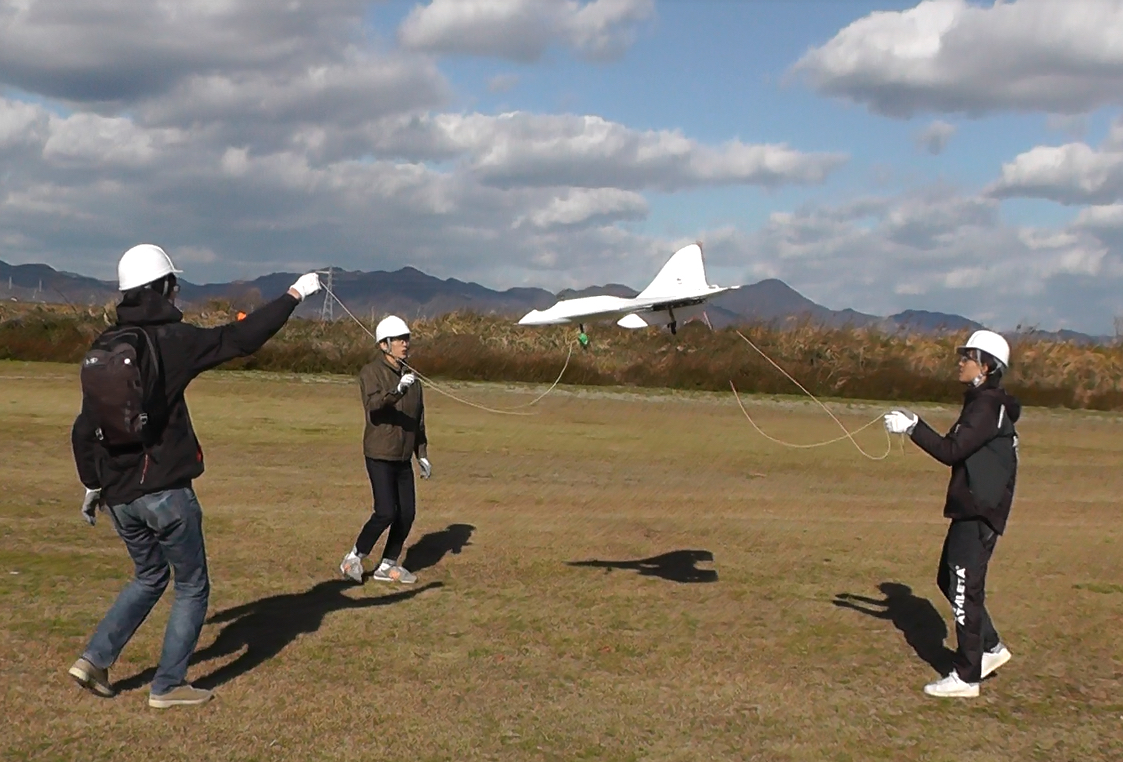
\includegraphics[clip,width=10cm,bb=0 0 1123 762]{./z_figure_files/chapter4/experiment.jpeg}
    \caption{Outdoor experiment under strong wind}
    \label{fig:flight_ex}
  \end{center}
\end{figure}

\begin{table} [htbp]
  \begin{center}
    \caption{Identified parameters}
    \label{tb:si_result}
    \begin{tabular}{|c||r|cc||r|} \hline
      $C_{L_0}$ & 0.1313 & & $C_{m_0}$ & 1.237 \\ \hline
      $C_{L_\alpha}$ & 0.7357 & & $C_{m_\alpha}$ & -0.04574 \\ \hline
      $C_{L_{\dot{\alpha}}}$ & -36.87 & & $C_{m_{\dot{\alpha}}}$ & -7.799 \\ \hline
      $C_{L_q}$ & 36.33 & & $C_{m_q}$ & 8.414 \\ \hline
      $C_{L_{\delta_e}}$ & -1.112 & & $C_{m_{\delta_e}}$ & 0.4092 \\ \hline
      $C_{L_k}$ & -4.070 & & $C_{m_k}$ & -7.505 \\ \hline
      $C_{D_0}$ & 0.2385 &&&\\ \hline
      $\kappa$ & 0.2228 &&&\\ \hline
      $C_{D_k}$ & 5.976 &&&\\ \hline
    \end{tabular}
  \end{center}
\end{table}

\begin{figure}[htbp]
	\begin{center}
		\begin{tabular}{c}
			\begin{minipage}{0.5\hsize}
				\begin{center}
					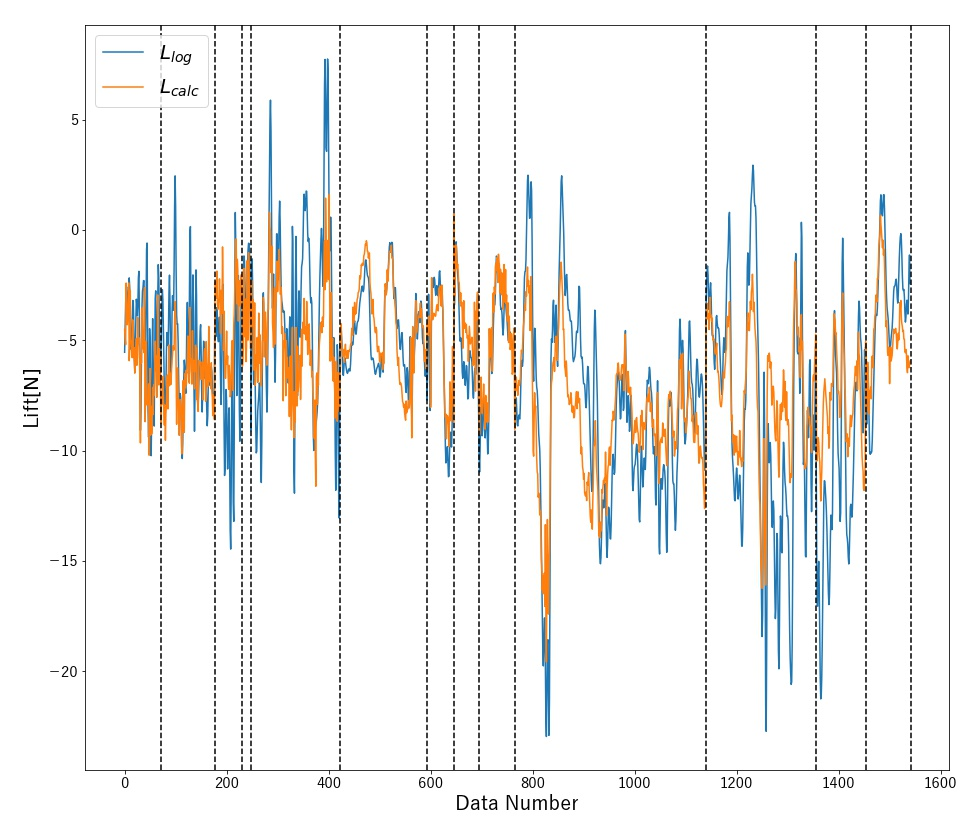
\includegraphics[clip,width=7.5cm,bb=0 0 864 654]{./z_figure_files/chapter4/L.jpeg}
					\caption{Reproduction of lift}
					\label{fig:L_re}
				\end{center}
			\end{minipage}
			\begin{minipage}{0.5\hsize}
				\begin{center}
					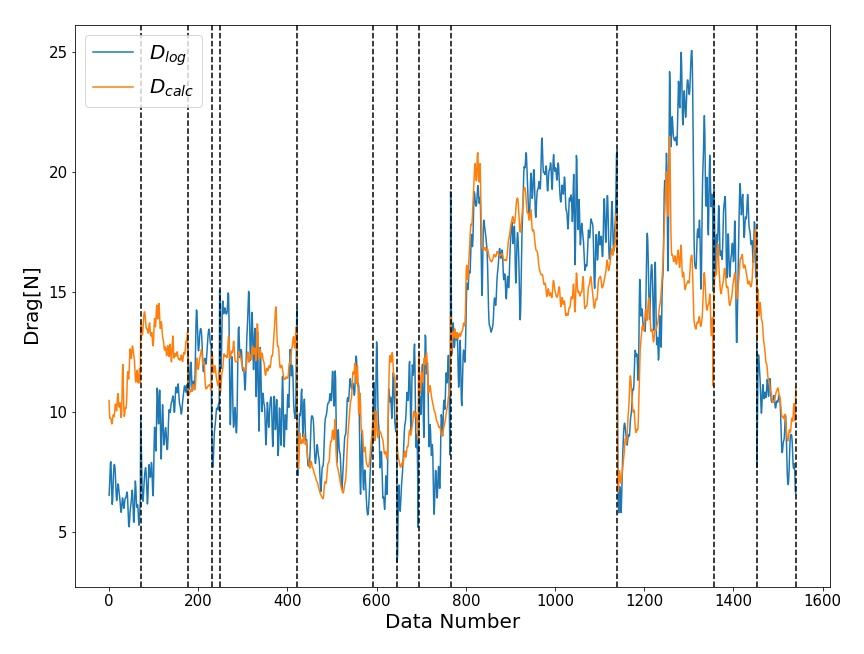
\includegraphics[clip,width=7.5cm,bb=0 0 864 654]{./z_figure_files/chapter4/D.jpeg}
					\caption{Reproduction of drag}
					\label{fig:D_re}
				\end{center}
			\end{minipage}
		\end{tabular}
	\end{center}
\end{figure}
\begin{figure}[H]
  \begin{center}
    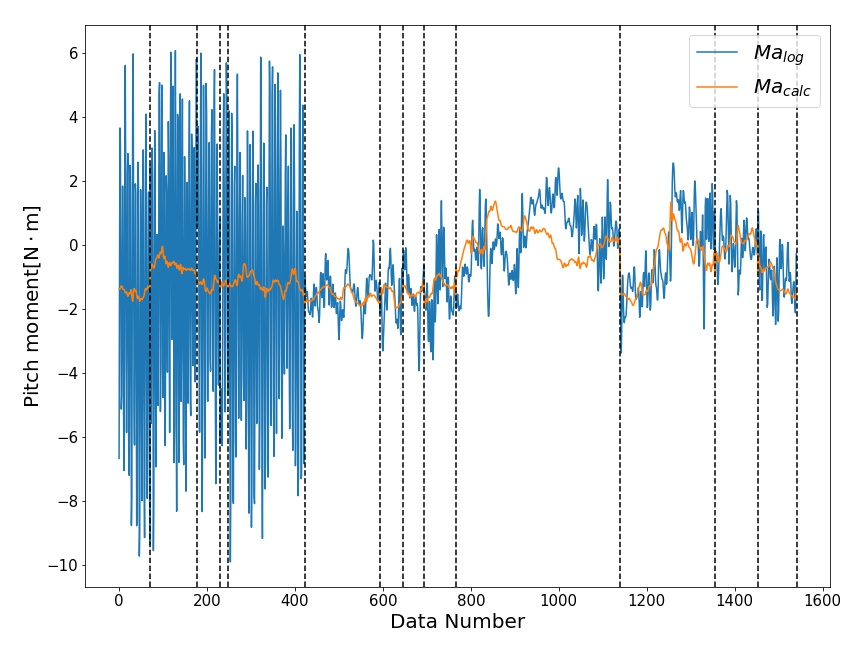
\includegraphics[clip,width=7.5cm,bb=0 0 864 654]{./z_figure_files/chapter4/Ma.jpeg}
    \caption{Reproduction of pitch moment}
    \label{fig:Ma_re}
  \end{center}
\end{figure}


% 実際の推定結果とそれに対する考察は,\ref{sec:airf_model_ver}節で行なう.
